\section{Induction \& Grammar}
You may have been taught induction through stories of falling 
dominos.  Good.  But what if induction was more like what we just did, climbing?
The domino illustration could bottle up the experience of climbing stairs.  
Now we climb trees and maybe mountains.
Setting up this induction was nothing more than a fragment of text but 
read through the lens of a grammar, e.g.\ PEMDAS, it came into a full form
as steps for recursion.

\index{parsing}
Parsing grammars in natural language is not always clarifying.  A simplistic
English grammar will often parse into cycles.
\begin{center}
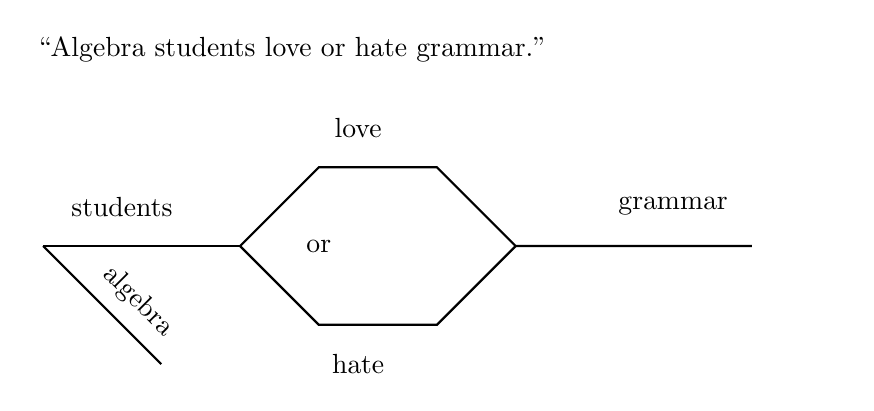
\begin{tikzpicture}
    \node[text width=4in] at (1,2) {``Algebra students love or hate grammar.''};
    \node at (-3,0) {students};
    \node[rotate=-45] at (-2.8,-1.2) {algebra};
    \node at (-0.5,-0.5) {or};
    \node at (0,1) {love};
    \node at (0,-2) {hate};
    \node at (4,0) {grammar};

    \draw[thick] (-4,-0.5) -- ++(2.5,0);
    \draw[thick] (-4,-0.5) -- ++(1.5,-1.5);
    \draw[thick] (-1.5,-0.5) -- ++(1,1) -- ++(1.5,0) -- ++(1,-1) -- ++(3,0);
    \draw[thick] (-1.5,-0.5) -- ++(1,-1) -- ++(1.5,0) -- ++(1,1);

\end{tikzpicture}
\end{center}
So our inductive climbs may one day need many routes, even go in cycles.
Fortunately, evaluating a formula has a precise algorithm without ambiguity. The
reason is that we had a rooted tree.  Trees have unique paths between any two
vertices. So if we start at the leaves we have a unique direction to reach the
root. 



\index{context-free}
That we got a tree in math formulas means we have a rather boring grammar, 
what Chompsky's \emph{Syntactic Structure} calls
\emph{context-free} grammars.\footnote{
    If an algebraist starts a talk with a story that ``...It was thought  all natural 
    languages were context-free until some obscure dialect in the alps or Africa was found...'', 
    then tune out until they return to equations.  
    Linguist never had such illusions. Even english is not context-free, read  James Higginbotham.} 
Don't be too disheartened.  Virtually every programming language has a 
context-free grammar and programs can communicate a lot of hefty ideas. 

\begin{quote}
    \textbf{Complex inductions can be specified by grammar.}
\end{quote}
